\documentclass{article}
\usepackage[utf8]{vietnam}
\usepackage{graphicx}
\usepackage{amsmath}
\usepackage{amssymb}
\usepackage{hyperref}
\usepackage{caption}
\usepackage{subcaption}
\usepackage[a4paper, total={6in, 8in}]{geometry}

\title{A gentle introduction to Deep Learning \\ \Large Report Lab Week 15-16-17-18}
\author{Ngọc Thuận - IPSAL LAB}
\date{April 2023}

\begin{document}

\maketitle
\begin{abstract}
Trong bài trước ta đã đi qua những khái niệm, thuật toán và một số mô hình cơ bản trong Machine Learning. Trong bài này ta sẽ nghiên cứu một số vấn đề chính trong Deep Learning. Bắt đầu từ những công cụ cơ bản như tích chập cho đến những mô hình học sâu cổ điển và hiện đại, cách xây dựng một mô hình học sâu, cuối cùng là đôi chút về fine-tuning trong transfer learning.    
\end{abstract}
\tableofcontents
\newpage
\section{Deep Learning là gì?}
Tôi vừa google `Deep Learning là gì?' để tìm kiếm hình ảnh minh họa phù hợp, nhưng có vẻ không tìm thấy, cho nên tôi sẽ nói chay vậy, một cách đơn giản thôi. Nếu định nghĩa như bài trước, Deep Learning là một nhánh con đang phát triển của Machine Learning thì có vẻ hơi `gợn'. Để hiểu được chữ `sâu', có lẽ sẽ dễ dàng hơn khi ta làm việc với chúng và định nghĩa điều đó thật chẳng dễ dàng.\\\\
Ta có thể hình dung một cách đơng giản như sau: Trong bài trước, khi nghiên cứu về MPLs - cách mạng neuron đa tầng, ta biết rằng việc thêm các tầng ẩn sẽ làm tăng độ phức tạp của mô hình và mô hình sẽ dễ khớp hơn đúng không? Càng nhiều tầng ẩn mô hình càng dễ khớp với dữ liệu trên tập huấn luyện và trực quan mà nói đa số nó cũng sẽ làm việc tốt trên tập kiểm định. Điều đó có thể giải thích rằng các đặc trưng sẽ được trích xuất càng kĩ nếu mô hình càng nhiều lớp, càng nhiều đặc trưng về một đối tượng, hay càng nhiều thông tin về đối tượng, ta càng xác định rõ được đối tượng cũng như bài toán liên quan đến đối tượng. Từ `sâu' ở đây là ở chiều sâu của mô hình.\\\\
Rõ ràng ta chỉ cần tăng chiều sâu mô hình MPLs lên là được đúng không? Nếu đơn giản như vậy thì ta chẳng cần đến khái niệm này! Thực tế, để tăng độ phức tạp của một mô hình MPLs là khó, đặc biệt với các tín hiệu đặc biệt như hình ảnh. Bởi mô hình càng sâu, số lượng tham số càng lớn. Giả sử rằng ta có bức ảnh $32 \times 32$, được trải phẳng làm đầu vào của một mô hình MPLs với các lớp lần lượt là $100, 200, 10$. Số lượng tham số sẽ là $32\times 32 \times100\times200\times10 = 204800000
$ gần 205 triệu tham số cho chỉ 3 lớp với bức ảnh phân giải thấp. Với số lượng tham số này CPU chắc đứt cả hơi mới ra được kết quả, vừa mất thời gian, mô hình cũng chưa đủ sâu và ta cũng đã bỏ qua những sự liên kết về không gian trong một bức ảnh.\\\\
Học sâu trong phạm vi bài này ta cũng chỉ nói chủ yếu về Thị giác máy tính, hay làm việc với dữ liệu hai chiều là các bức ảnh. Khởi nguồn cho tên gọi này cũng bắt nguồn từ chúng. Như trên ta đã thấy rõ mặt hạn chế của phương pháp cổ điển, có ý tưởng đấy nhưng mà không thể nào làm được theo các phương pháp cũ!\\\\
Và giải pháp ở đây là các tầng tích chập (convolutional layers) thay thế cho các tầng kết nối đầy đủ (dense layers/ fully conected layers). Mô hình LeNet ra đời năm 1998 là mô hình mạng neuron tích chập đầu tiên. Song phải thật sự đến 2012 với AlexNet thì khái niệm học sâu mới thật sự được rõ ràng!\\\\
Để bắt đầu ta sẽ đi vào tìm hiểu về cấu tạo của một tầng tích chập sẽ như thế nào!
\section{Tầng tích chập}
\subsection{Từ MPLs tới CNN}
Giả sử ảnh đầu vào vẫn giữ kích thước 2 chiều: $h\times w$ và các đặc trưng trích xuất được cũng ở dạng hai chiều. Tức là đây là một tầng kết nối đầy đủ với mỗi nút là một điểm ảnh của tầng đầu ra. Ta có thể kí hiệu ảnh đầu vào là \textbf{x}, ma trận đầu ra là \textbf{h}.\\\\
Giống như một nút trong MPLs, 1 điểm ảnh ở đầu ra cũng được tính tương tự như sau:
\begin{equation}
    \textbf{h}[i,j] = \textbf{u}[i,j]+\sum_{k,l}\textbf{W}[i,j,k,l]\textbf{x}[k,l]
    \label{eq1}
\end{equation}
tổng có trọng số của các nút ở đầu vào.\\\\
Đổi biến $k = i+a, l = j+b$, ta có:
\begin{equation}
    \textbf{h}[i,j] = \textbf{u}[i,j]+\sum_{a,b}\textbf{V}[i,j,a,b]\textbf{x}[i+a,j+b]
    \label{eq2}
\end{equation}
Giả sử \textbf{u, V} không phụ thuộc vào $i,j$ (tính bất biến), ta thu được:
\begin{equation}
    \textbf{h}[i,j] = u+\sum_{a,b}\textbf{V}[a,b]\textbf{x}[i+a,j+b]
    \label{eq3}
\end{equation}
Giả sử $\textbf{V}[a,b]$ chỉ phụ thuộc vào các điểm ảnh ở lân cận (tính cục bộ). Khi đó ta thu được kết quả cuối cùng
\begin{equation}
        \textbf{h}[i,j] = u+\sum_{a=-\Delta}^{\Delta}\sum_{b = -\Delta}^{\Delta}\textbf{V}[a,b]\textbf{x}[i+a,j+b]
    \label{eq4}
\end{equation}
Công thức (\ref{eq4}) chính là phép tích chập hai chiều ta đã biết!\\\\
\underline{Nhận xét}
\begin{enumerate}
    \item Với tính bất biến, tất cả các mảng nhỏ trong ảnh đều được xử lí theo cùng một cách.
    \item Với tính cục bộ, chỉ một vùng lân cận nhỏ các điểm ảnh sẽ được sử dụng trong tính toán. Việc này có lợi ích lớn, tạo thành các ma trận \textit{thưa}, giảm đáng kể tham số.
    \item Với thay đổi trên thì sẽ giữ được sự tương quan giữa các pixels ảnh đầu vào.
\end{enumerate}
\subsection{Phép tích chập}
Phần này tôi đã giới thiệu trong bài \textit{Các phép lọc không gian}, xin phép sẽ không nhắc lại. Tuy nhiên có một số khái niệm mới ta cần để ý:
\subsubsection*{Tầng tích chập}
Output của 1 tầng tích chập được gọi là feature maps/receptive feilds. \\\\
Cấu trúc của một tầng tích chập về bản chất chính là như phần trên. Khi đó bộ lọc/hạt nhân của ta chính là các tham số cần được học.
\subsection{Đệm và sải bước}
Để điều chỉnh kích thước của đầu ra, ta có thêm khái niệm đệm (padding) và sải bước (stride).\\\\
Giả sử kích thước của đầu vào là $n_h \times n_w$ và kích thước của hạt nhân là $k_h \times k_w$, kích thước của đầu ra sẽ là:
$$(n_h-k_h+1)\times(n_w-k_w+1)$$
\subsubsection{Đệm}
Nếu chúng ta chèn thêm tổng cộng $p_h$ hàng đệm (phân nửa phía trên và phân nữa phía dưới), $p_w$ cột đệm (phân nửa bên trái và phân nửa bên phải) thì kích hước đầu ra sẽ là:$$(n_h-k_h+p_h+1)\times(n_w-k_w+p_w+1)$$
Cách sử dụng ta có thể tham khảo trong hình \ref{fig1}
\begin{figure}[ht!]
    \centering
    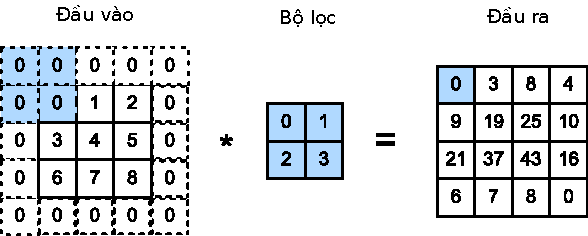
\includegraphics[width = 0.7\linewidth]{conv-pad.pdf}
    \caption{Tương quan chéo hai chiều khi thực hiện đệm. Phần tô đậm là các phần tử của mảng đầu vào và hạt nhân được sử dụng để tính phần tử đầu ra thứ nhất. DiveintoDeeplearning}
    \label{fig1}
\end{figure}
\phantom{a}\\
\underline{Lưu ý:}
\begin{enumerate}
    \item Đặt $p_h = k_h-1$, $p_w = k_w - 1$, đầu vào có kích thước không đổi.
    \item Các bộ lọc thường sử dụng với kích thước lẻ, điều này hữu ích khi ta đệm sao cho đầu ra không thay đổi kích thước. Khi đó ta sẽ được một tương ứng giữa đầu vào và đầu ra.
\end{enumerate}
\subsubsection{Sải bước}
Nếu ta di chuyển từ trái sang phải mỗi lượt là $s_w$ pixels, từ trên xuối là $s_h$. Đầu ra sẽ có kích thước tương ứng:
$$(n_h-k_h+p_h+s_h)/s_h\times(n_w-k_w+p_w+s_w)/s_w$$
Cách sử dụng ta có thể xem trong hình \ref{fig2}
\begin{figure}[ht!]
    \centering
    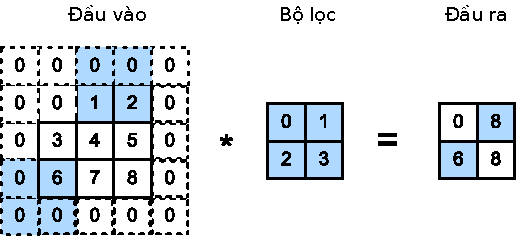
\includegraphics[width = 0.6\linewidth]{conv-stride.pdf}
    \caption{Phép tương quan chéo với sải bước 3 theo chiều dài và và 2 theo chiều rộng. Phần tô đậm là các phần tử đầu ra, các phần tử đầu vào và bộ lọc được sử dụng để tính các đầu ra này. DiveintoDeeplearning}
    \label{fig2}
\end{figure}
\subsection{Đa kênh đầu vào đa kênh đầu ra}
Như ta đã biết thì ảnh của ta thường là các ảnh RGB là chủ yếu, 3 kênh. Khi đó câu hỏi đặt ra là liệu có tích chập được trong trường hợp đó không? Và câu hỏi tương tự rằng liệu 1 phép tích chập có thể có nhiều đầu ra không?
\subsubsection{Đa kênh đầu vào}
Rõ ràng để làm được điều này, ta cần số lượng hạt nhân bằng với số lượng kênh, tức là một hạt nhân sẽ thực hiện tích chập cho một kênh. Sau đó ta tổng hợp lại kết quả bằng cách cộng các đầu ra lại với nhau. Hình \ref{fig3} minh họa cho điều này
\begin{figure}[ht!]
    \centering
    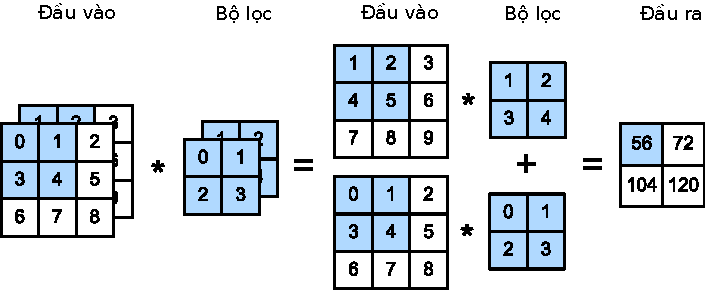
\includegraphics[width = 0.7\linewidth]{conv-multi-in.pdf}
    \caption{Phép tính tương quan chéo với hai kênh đầu vào. Phần tô đậm là phần tử đầu ra đầu tiên cùng các phần tử của mảng đầu vào và bộ lọc được sử dụng trong phép tính đó. DiveintoDeeplearning}
    \label{fig3}
\end{figure}
\subsubsection{Đa kênh đầu ra}
Phần này ta cần đi chậm lại một chút. Trong các kiến trúc mạng neuron phổ biến nhất, ta thường tăng kích thước chiều kênh khi tiến sâu hơn trong mạng, đồng thời giảm độ phân giải không gian để đánh đổi \textit{chiều kênh} sâu này. Theo trực giác, ta có thể xem mỗi kênh tương ứng với một tập các đặc trưng khác nhau, tuy nhiên cá biển diễn này không được học đập lập mà được tối ưu hóa để có ích khi kết hợp với nhau. Vì vậy, có thể việc phát hiện biên sẽ được học bởi một vài kênh thay vì chỉ một kênh duy nhất.\\\\
Như ở mục trên, một bức ảnh có đầu vào $c_i$ kênh cần một bộ lọc có kích thước $c_i\times k_h\times k_w$. Giả sử ta muốn có $c_o$ kênh đầu ra sau tầng tích chập thì bộ lọc tích chập của ta cần có kích thước là $c_o \times c_i \times k_h \times k_w$.
\subsubsection{Tầng tích chập 1x1}
Trực quan ta thấy phép tích chập này vô dụng, vì dường như ta chả lấy được thông tin gì từ các điểm ảnh lân cận. Tuy nhiên, chúng lại là thành phần được sử dụng khá phổ biến trong các mô hình mạng sâu phức tạp.\\\\
Do cửa sổ có kích thước tối thiểu nên so với các tầng tích chập lớn hơn, chúng mất đi khả năng nhận dạng các khuôn mẫu chứa các tương tác giữa các phần tử liền kề theo chiều cao và chiều rộng, chúng chỉ có tác dụng theo chiều kênh. Do đó ý nghĩa của nó là để điều chỉnh số lượng kênh giữa các tầng của mạng và kiểm soát độ phức tạp của mô hình.
\begin{figure}[ht!]
    \centering
    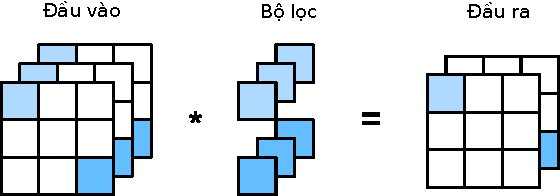
\includegraphics[width = 0.7\linewidth]{conv-1x1.pdf}
    \caption{Phép tính tương quan chéo sử dụng bộ lọc tích chập  1×1
  với 3 kênh đầu vào và 2 kênh đầu ra. Các đầu vào và các đầu ra có cùng chiều cao và chiều rộng. DiveintoDeeplearning}
    \label{fig4}
\end{figure}
\section{Tầng gộp}
Tầng gộp cũng là một trong những thành phần không thể thiếu trong các mạng neuron tích chập. Tầng gộp có nhiệm vụ là giảm dần độ phân giải không gian của các biểu diễn ẩn, tổng hợp thông tin lại để khi càng đi vào sâu mạng, vùng tiếp nhận (ở đầu vào) ảnh hưởng đến mỗi nút ẩn càng lớn.\\\\
Nhiệm vụ cuối cùng thường là trả lời một câu hỏi nào đó về toàn bộ tấm ảnh, ví dụ như: trong ảnh có mèo không? Vậy nên các nút của tầng cuối cùng thường cần phải chịu ảnh hưởng của toàn độ đầu vào. Bằng cách dần gộp thông tin lại để tạo ra cá ánh xạ đặc trưng thưa dần, ta sẽ học được một biểu diễn toàn cục, trong khi vẫn có thể giữ nguyên toàn bộ lợi thế đến từ các tầng tích chập xử lí trung gian.\\\\
Tầng gộp có tính bất biến với phép tịnh tiến trong một chừng mực nào đó giảm độ nhạy cảm của các tầng tích chập đối vói vị trí.
\subsection{Gộp trung bình và Gộp cực đại}
Tầng gộp cũng giống như tầng tích chập, tuy nhiên tầng gộp \textit{không có} bộ lọc như tầng tích chập. Hình \ref{fig5} minh họa cho cách sử dụng.
\begin{figure}[ht!]
    \centering
    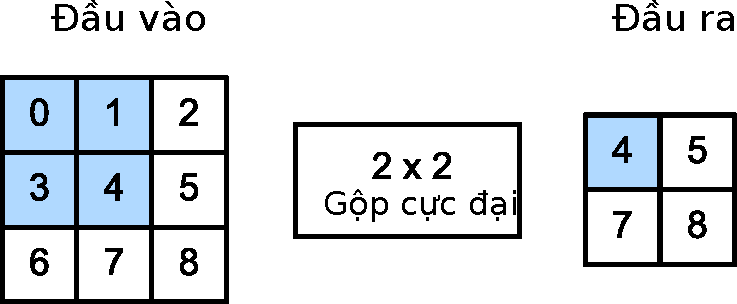
\includegraphics[width = 0.5\linewidth]{pooling.pdf}
    \caption{Gộp cực đại với cửa sổ có kích thước  2×2
 . Các phần tô đậm thể hiện phần tử đầu ra đầu tiên và phần tử đầu vào được dùng để tính toán:  max$(0,1,3,4)=4$
 . DiveintoDeeplearning}
    \label{fig5}
\end{figure}
\subsection{Đệm và sải bước}
Trong tầng gộp cũng có khái niệm đệm và sải bước, và nó giống y bên tích chập.
\subsection{Với đầu vào đa kênh}
Bên cạnh đệm và sải bước, tầng hộp cũng hỗ trợ cho việc gộp tầng đầu vào đa kênh. Tuy nhiên, ở đây lại khá khác so với tầng tích chập. Nếu ở các tầng tích chập, đầu ra của đa kênh đầu vào sẽ là tổng các kênh đầu ra ứng với các kênh đầu vào thì ở tầng gộp các kênh đầu ra sẽ giữ nguyên, tầng gộp sẽ áp dụng lên từng kênh một cách riêng biệt!
\section{Một số mô hình mạng neuron tích chập}
Trên là tất cả những gì cần để xây dựng một mô hình mạng neuron tích chập. Sau đây chúng ta sẽ lướt qua một vài mạng neuron tích chập kinh điển đã đánh dấu những bước phát triển của Deep Learning.
\subsection{LeNet}
Đây là mô hình mạng neuron tích chập đầu tiên được triển khai thành công bởi Yann LeCun và các cộng sự vào những năm 1980s.\\\\
Tuy nhiên vào thời điểm ra mắt, dù đạt được kết quả tương đối tốt, song mạng neuron tích chập vẫn bị nhìn bằng con mắt hoài nghi và chưa được thực sự chú ý và quan tâm. Có lẽ bởi những không tường minh trong cấu trúc cũng như kết quả cũng chưa quá nổi bật so với các thuật toán \textit{máy vector hỗ trợ}.
\\\\
Cấu trúc của LeNet như hình \ref{fig6}. Dạng vắn tắt ở hình \ref{fig7}
\begin{figure}[ht!]
    \centering
    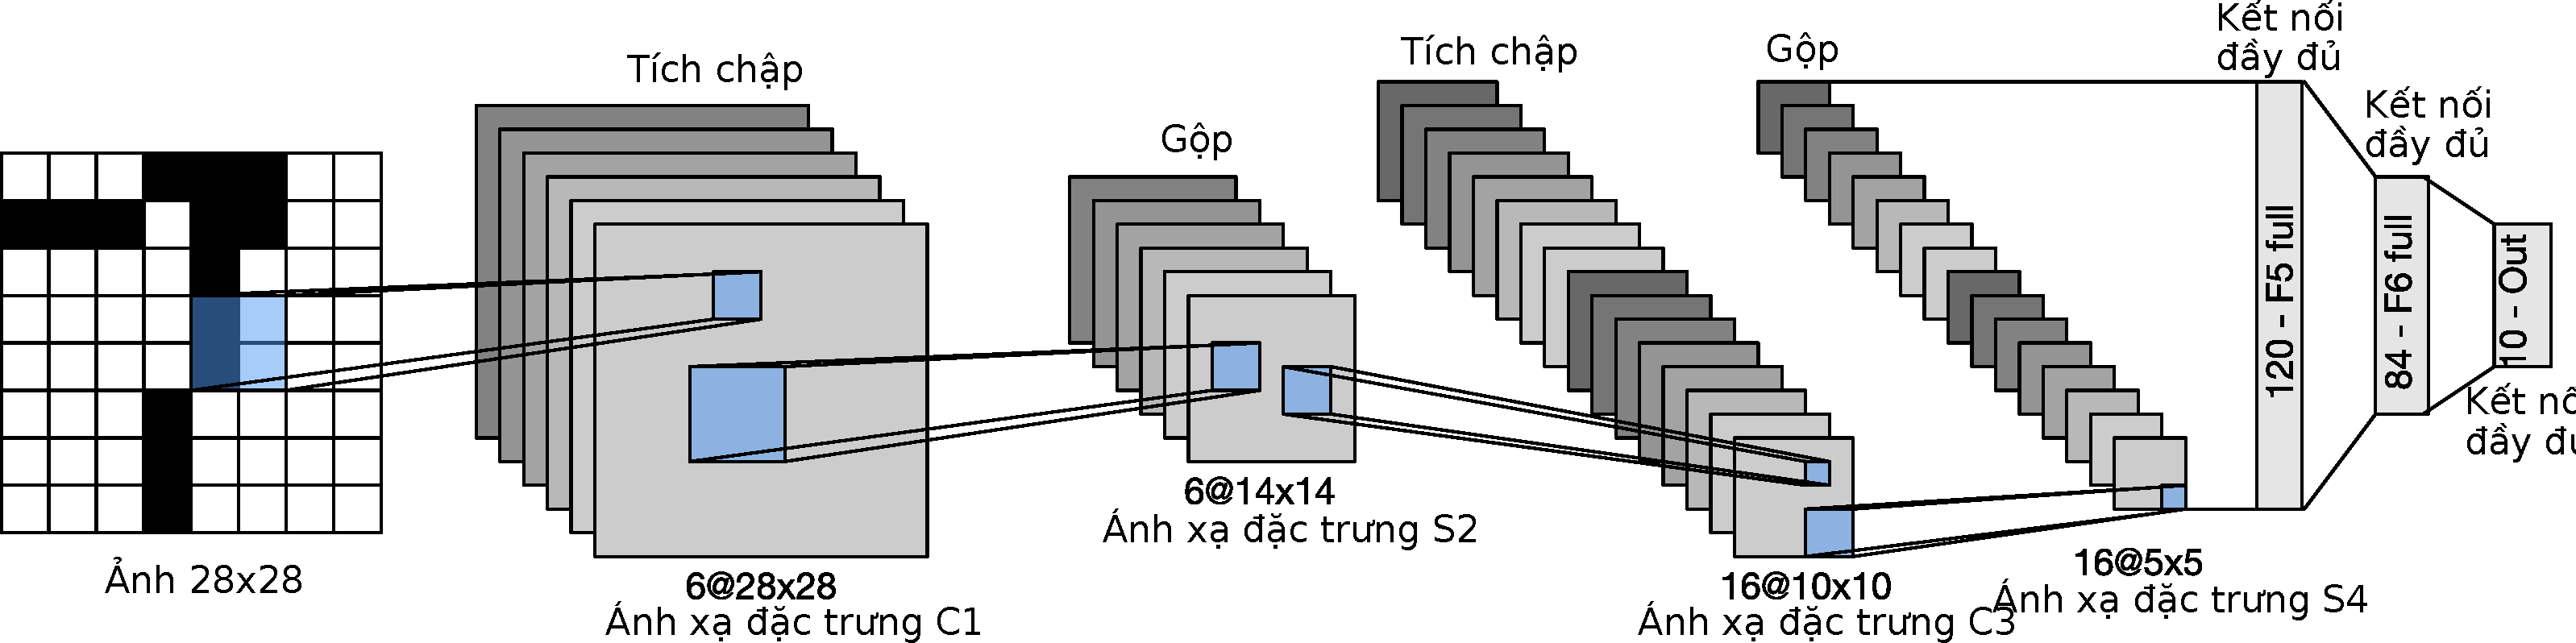
\includegraphics[width = 0.8\linewidth]{lenet.pdf}
    \caption{Dòng dữ liệu trong LeNet 5. Đầu vào là một chữ số viết tay, đầu ra là một xác suất đối với 10 kết quả khả thi. DiveintoDeeplearning}
    \label{fig6}
\end{figure}
\begin{figure}[ht!]
    \centering
    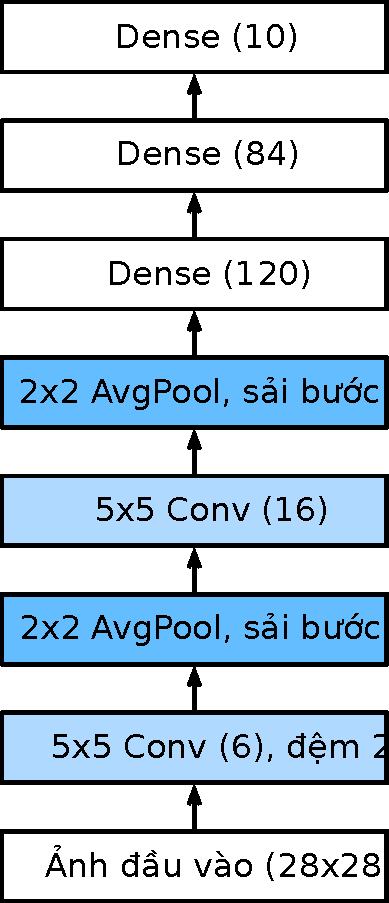
\includegraphics[width = 0.2\linewidth]{lenet-vert.pdf}
    \caption{Kí hiệu vắn tắt cho mô hình LeNet 5. DiveintoDeeplearning}
    \label{fig7}
\end{figure}
\subsection{AlexNet}
AlexNet, mạng CNN quy mô lớn đầu tiên được triển khai đã đánh bại các phương pháp thị giác máy tính truyền thống trong một thử thách quy mô lớn (ImageNet Challenge 2012).
\begin{figure}[ht!]
    \centering
    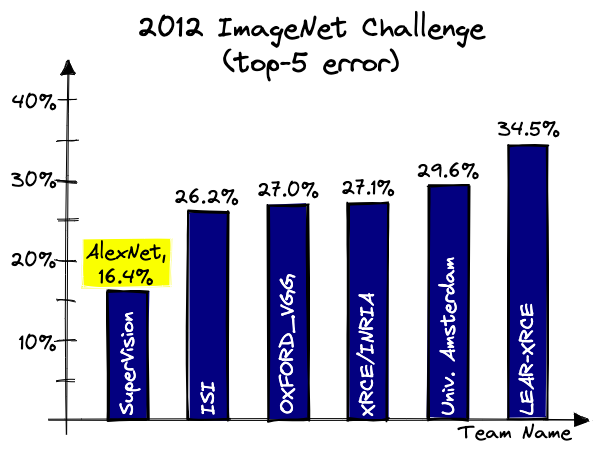
\includegraphics[width = 0.5\linewidth]{imagenet-5.png}
    \caption{Top 5 trong ImageNet Challenge 2012}
    \label{fig8}
\end{figure}
\phantom{a}\\
Cấu trúc của mạng AlexNet như hình \ref{fig9}
\begin{figure}[ht!]
    \centering
    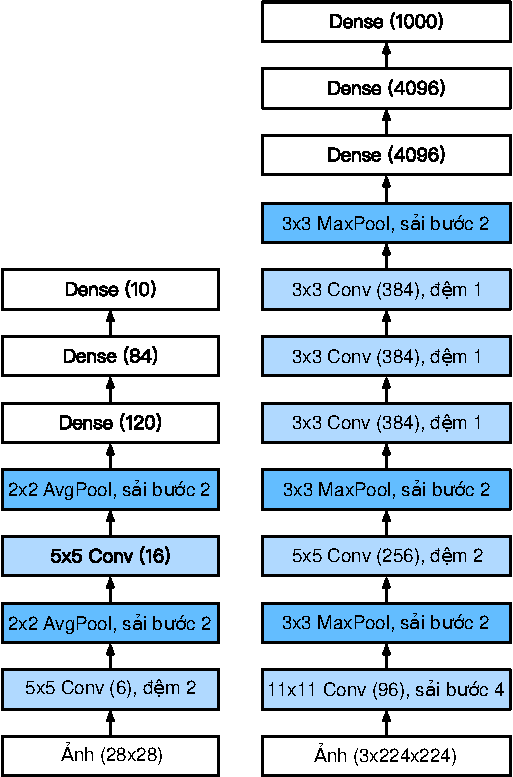
\includegraphics[width = 0.4\linewidth]{alexnet.pdf}
    \caption{LeNet (trái) và AlexNet (phải). DiveintoDeeplearning}
    \label{fig9}
\end{figure}
\phantom{a}\\
Về trực quan AlexNet không quá khác biệt so với LeNet, tuy nhiên có một vài khác biệt nổi bật đã thay đổi hoàn toàn cuộc chơi:
\begin{enumerate}
    \item Hàm kích hoạt ReLU
    \item Sử dụng 2 GPUs để huấn luyện
    \item Điều chuẩn Dropout
    \item Tiền xử lí (AlexNet đã bổ sung rất nhiều kĩ thuật tăng cường ảnh, chẳng hạn như lật, cắt hay thay đổi màu sắc. Điều này giúp cho mô hình trở nên mạnh mẽ hơn, cùng với đó kích thước dữ liệu lớn hơn giúp làm giảm hiện tượng quá khớp một cách hiệu quả)
\end{enumerate}
Hơn 20 năm, từ một nghiên cứu tưởng chừng bị ngủ quên, đến một cuộc cách mạng trong học máy. AlexNet đã chứng minh được tính hiệu quả của mạng neuron tích chập, giúp cho GPU được tỏa sáng mặc cho chúng một hướng phát triển mới đầy tiềm năng và cao cả! Thật sự AlexNet đã cứu Nvidia!!!
\subsection{VGG}
Mặc dù AlexNet đã chứng minh được tính hiệu quả của các mạng neuron tích chập, song nó lại không cung cấp một khuôn mẫu chung để định hướng nghiên cứu sau này trong việc thiết kế các mạng mới.\\\\
Việc thiết kế kiến trúc các mạng neuron đã phát triển theo hướng ngày một trừu tượng hơn. Điển hình là việc các nhà nghiên cứu đã thay đổi suy nghĩ từ quy mô riêng lẻ sang các tầng, và giờ đây là các khối chứa các tầng lặp lại theo khuôn mẫu.\\\\
Ý tưởng sử dụng các khối lần đầu tiên xuất hiện trong mạng VGG, được đặt theo tên của nhóm VGG thuộc Đại học Oxford. Sử dụng bất kì các framework học sâu hiện đại nào với vòng lặp và chương trình con để xây dựng các cấu trúc lặp lại này là tương đối dễ dàng.\\\\
Cấu trúc của VGG ở trên hình \ref{fig10}
\begin{figure}[ht!]
    \centering
    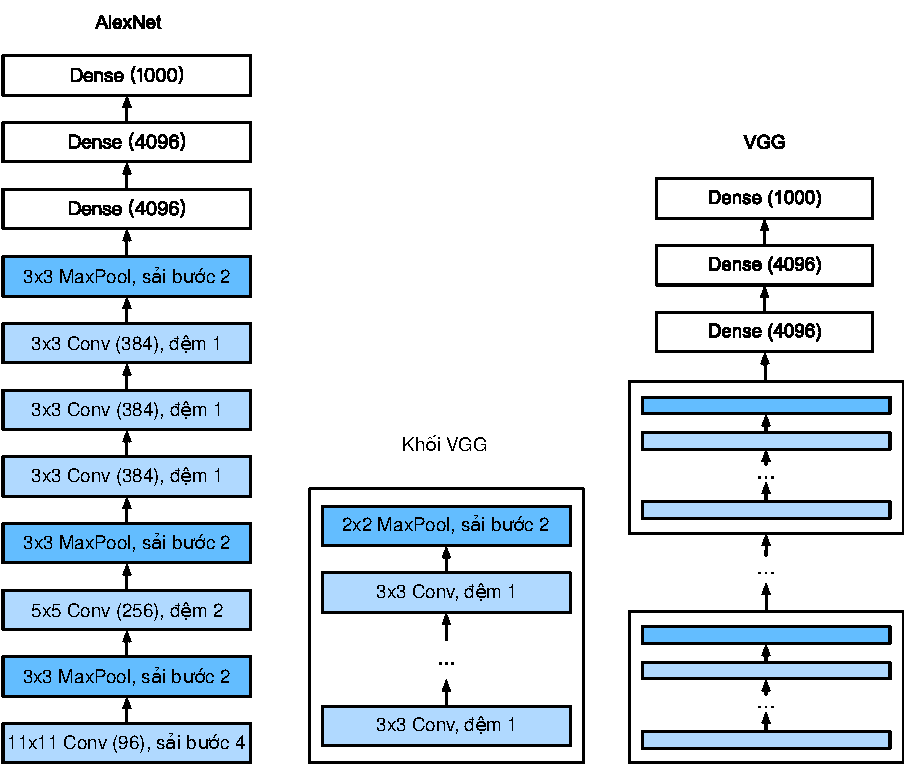
\includegraphics[width = 0.6\linewidth]{vgg.pdf}
    \caption{Thiết kế mạng từ các khối cơ bản. DiveintoDeeplearning}
    \label{fig10}
\end{figure}
\subsection{Mạng trong mạng (Network in Network - NiN)}
Thật ra, nếu nhìn kĩ ta sẽ thấy 3 mô hình trên về bản chất chả khác nhau, ngoại trừ chiều sâu và sau đó hậu xử lí bằng các tầng kết nối đầy đủ. Việc này rõ ràng có thể làm mất đi cấu trúc không gian của biểu diễn. NiN đề xuất một giải pháp khác: Gộp trung bình toàn cục (tính trung bình cộng tất cả các vị trí sau khi giảm số lượng kênh xuống bằng với số lượng đầu ra mong muốn).\\\\
Ngoài đề xuất trên, trong các khối NiN có cấu thành từ nhiều tầng tích chập $1 \times 1$, tăng tính phi tuyến trên điểm ảnh.\\\\
Những đề xuất này đã giúp giảm hiện tượng quá khớp, giảm số lượng tham số và ảnh hưởng lớn tới thiết kế của các mạng neuron tích chập sau này.
\\\\
Cấu trúc của NiN, hình \ref{fig11}
\begin{figure}[ht!]
    \centering
    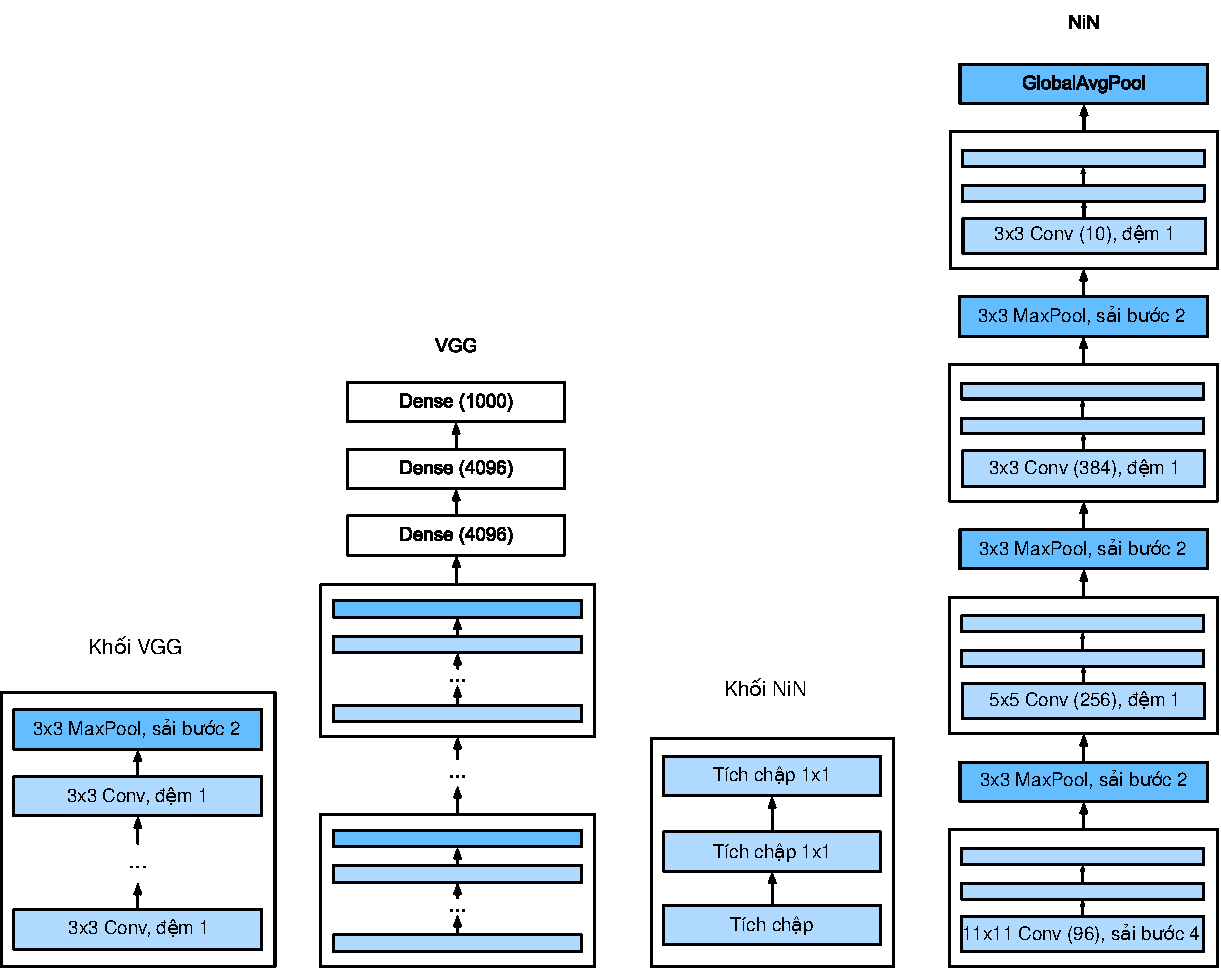
\includegraphics[width = 0.8\linewidth]{nin.pdf}
    \caption{Hình bên trái biểu diễn cấu trúc mạng của AlexNet và VGG, và hình bênh phải biểu diễn cấu trúc mạng của NiN. DiveintoDeeplearning}
    \label{fig11}
\end{figure}
\subsection{GoogLeNet}
GoogLeNet ra đời tập trung trả lời câu hỏi: kích thước nào của bộ lọc tích chập là tốt nhất? Bởi lẽ các mạng phổ biến trước đấy đều chọn các bộ lọc một cách đầy trực quan. Và GoogLeNet đề xuất việc kết hợp tất cả các bộ lọc lại, một cách phù hợp, có thể sẽ hiệu quả. 
\subsubsection*{Khối Inception}
Cái tên có lẽ được lấy cảm hứng từ bộ phim \textit{Inception (2010)} của Christopher Nolan, "\textit{We need to go deeper}". Khối Inception đề xuất ý tưởng sử dụng 4 nhánh song song với các bộ lọc khác nhau, sau đó tổng hợp thông tin lại ở tầng đầu ra. (hình \ref{fig12})
\begin{figure}
    \centering
    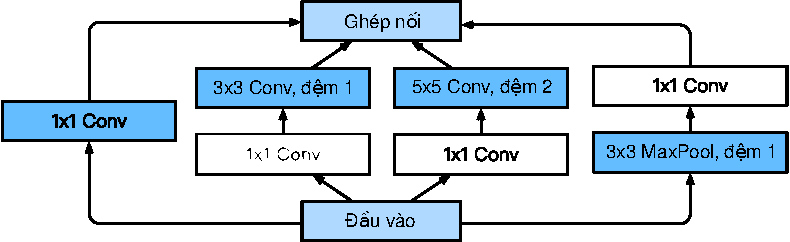
\includegraphics[width = 0.7\linewidth]{inception_block.pdf}
    \caption{Cấu trúc của khối Inception. DiveintoDeeplearning}
    \label{fig12}
\end{figure}
\phantom{a}\\
Ở đây ta thấy lại các tầng tích chập $1\times 1$ trong khối NiN. Chúng có tác dụng để điều chỉnh số kênh vào và ra, quản lí độ phức tạp của mô hình.
\\\\
Hình \ref{fig13}, mô hình GoogLeNet đầy đủ
\begin{figure}
    \centering
    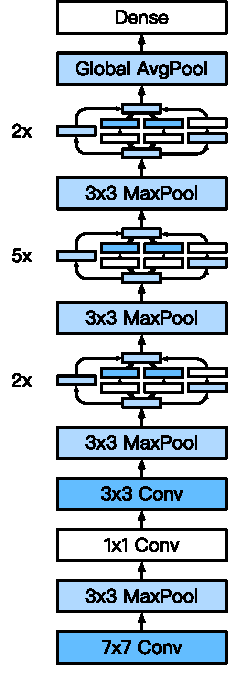
\includegraphics[width = 0.25\linewidth]{inception-full.pdf}
    \caption{Mô hình GoogLeNet đầy đủ. DiveintoDeeplearning}
    \label{fig13}
\end{figure}
\phantom{a}\\
Mô hình GoogLeNet, cũng như các phiên bản kế tiếp của nó, là một trong những mô hình hiệu quả nhất trên ImageNet, với độ chính xác tương tự trên tập kiểm tra nhưng độ phức tạp tính toán lại thấp hơn. Điều này truyền cảm hứng cho sự thiết kế của nhiều mạng thế hệ sau, trong đó có ResNeXtNet ta sẽ đề cập đến sau!

\subsection{Mạng phần dư (ResNet)}
Trực quan mà nói, ta nghĩ rằng mạng càng sâu thì độ chính xác càng cao đúng không? Tuy nhiên điều này không phải lúc nào cũng đúng, thậm chí còn có thể tệ đi. Câu hỏi được đặt ra là ta phải thêm các tầng, khối như thế nào để chắc chắn sẽ tăng tính biểu diễn thay vì chỉ một chút khác biệt?\\\\
Trước tiên ta cần hiểu một số lí thuyết cơ bản.
\subsubsection{Các lớp hàm số}
\begin{figure}
    \centering
    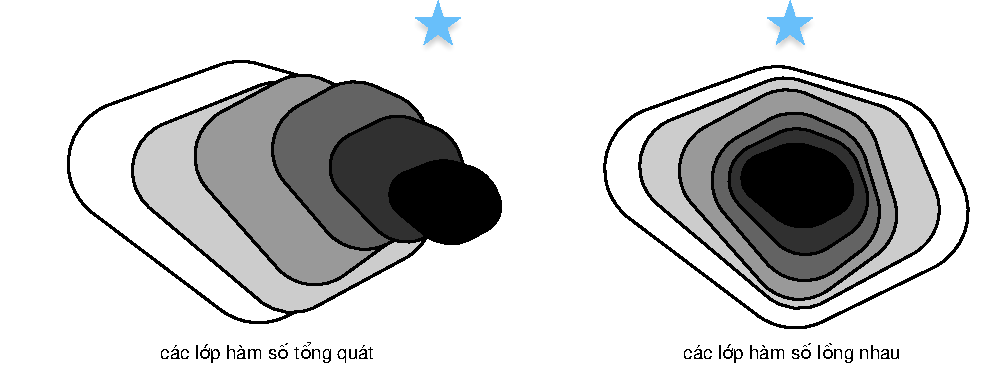
\includegraphics[width = 0.7\linewidth]{functionclasses.pdf}
    \caption{Hình trái: Các lớp hàm số tổng quát. Khoảng cách đến hàm cần tìm  $f^{*}$ (ngôi sao), trên thực tế có thể tăng khi độ phức tạp tăng lên. Hình phải: với các lớp hàm số lồng nhau, điều này không xảy ra. DiveintoDeeplearning}
    \label{fig14}
\end{figure}
\phantom{a}\\
Trong hình \ref{fig14}, ta có thể hiểu trực quan, khi ta thêm các tầng/khối để tăng độ phức tạp cho mô hình, giống như việc ta đang mơ rộng lớp các hàm mà mô hình có thể đạt được. Như hình bên trái, nếu ta cứ làm bừa, mô hình có thể sẽ ngày càng xa so với mục tiêu, điều này đôi khi còn tệ hơn. Điều này có thể giải thích do hàm đơn giản nhất trong một tầng lúc đó là hàm null $f(x) = 0$, nếu mục tiêu đi lệch thì kết quả là về 0! Do đó ResNet đề xuất hàm đơn giản nhất là $f(x) = x$, tức là mô hình mới hiệu quả ít nhất bằng mô hình ban đầu.\\\\
Cách suy nghĩ này khá trừu tượng nhưng lại dẫn đến một lời giải đơn giản đáng ngạc nhiên: khối phần dư (\textit{Residual block}). Với ý tưởng này, ResNet đã dành chiến thẳng trong ImageNet Challenge 2015. 
\subsubsection{Khối phần dư}
Cấu trúc của khối phần dư, hình \ref{fig15}
\begin{figure}
    \centering
    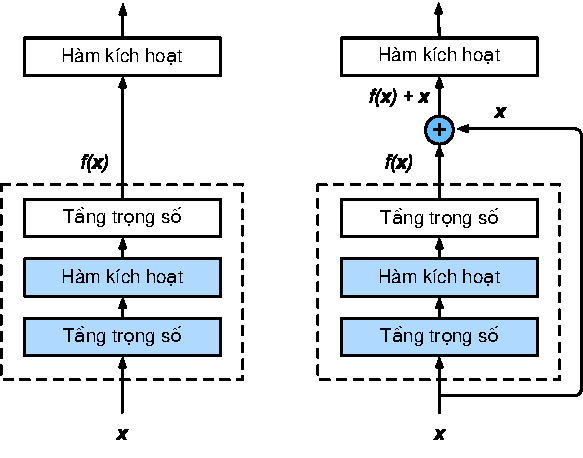
\includegraphics[width = 0.6\linewidth]{residual-block.pdf}
    \caption{Sự khác biệt giữa một khối thông thường (trái) và một khối phần dư (phải). Trong khối phần dư, ta có thể nối tắt các tích chập. DiveintoDeeplearning}
    \label{fig15}
\end{figure}
\phantom{a}\\
Kí hiệu đầu vào là \textbf{x}. Giả sử ánh xạ lý tường muốn học được là $f(\textbf{x})$, và được dùng làm đầu vào của hàm kích hoạt. Phần nằm trong viền nét đứt bên trái phải khớp trục tiếp với ánh xạ $f(\textbf{x})$. Đầu ra sẽ là $f(\textbf{x})+x$, nếu $f(\textbf{x}) = 0$ thì kết quả sẽ như ban đầu!
\subsection{Khối ResNet}
\begin{figure}
    \centering
    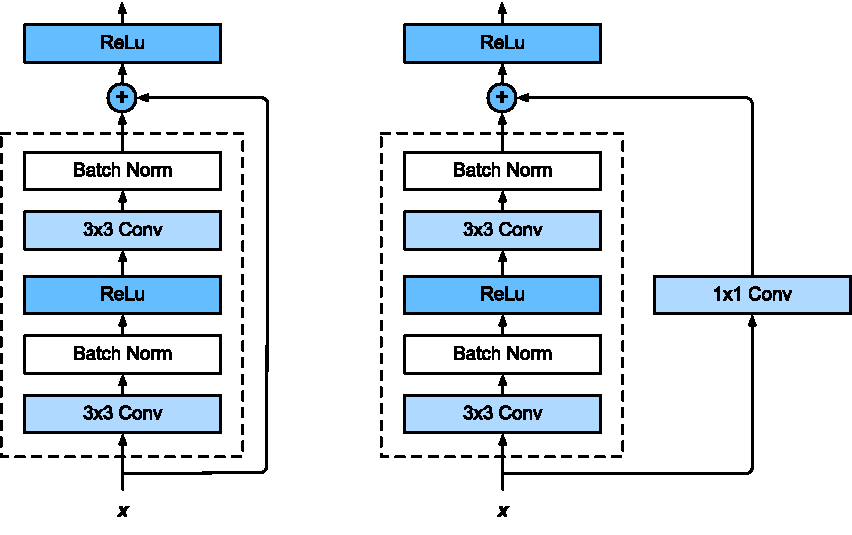
\includegraphics[width = 0.7\linewidth]{resnet-block.pdf}
    \caption{Trái: khối ResNet thông thường; Phải: Khối ResNet với tầng tích chập 1x1. DiveintoDeeplearning}
    \label{fig16}
\end{figure}
\phantom{a}\\
Cấu trúc của khối ResNet, hình \ref{fig16}. Có hai khối, một khối thông thường và một khối có tầng tích chập $1\times1$. Một điều mới ở khối ResNet là \textit{Chuẩn hóa theo Batch - Batch Normalization} (Đưa các mẫu về chuẩn tắc, điều này giúp cân bằng hệ số, tăng tốc độ hội tụ trong mạng).
\begin{figure}
    \centering
    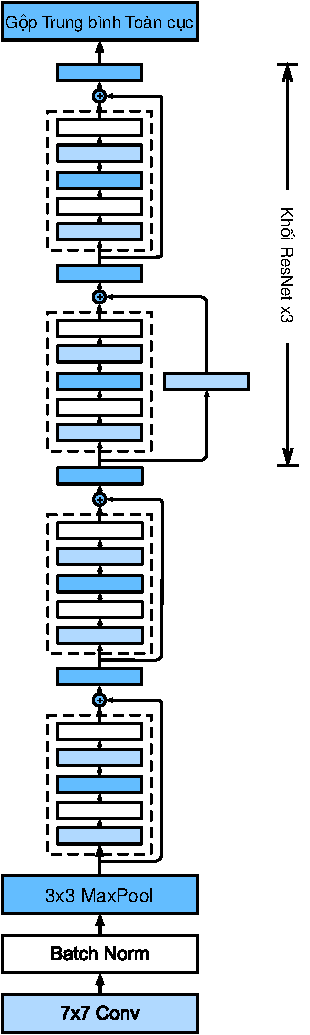
\includegraphics[width = 0.3\linewidth]{ResNetFull.pdf}
    \caption{ResNet-18. DiveintoDeeplearning}
    \label{fig17}
\end{figure}
\phantom{a}\\\\
Cấu trúc đầy đủ của ResNet, hình \ref{fig17}\\\\
Tổng quan thì, ResNet là một mô hình khá lí tưởng và phổ biến nhất hiện nay. Những đề xuất của nó trở thành tiêu chuẩn để thiết kế các mạng neuron tích chập sâu sau này.
\subsubsection{ResNeXt}
Lấy ý tưởng từ khối Inception, thông tin thu được từ nhiều khối độc lặp, áp dụng cho khối ResNet ta thu được ResNeXt. Khác với sự đa dạng về các phép biến đổi trong Inception, ResNeXt tất cả các nhánh đều giống nhau, do đó hạn chế việc phải điều chỉnh bằng tay trên mỗi nhánh.
\begin{figure}
    \centering
    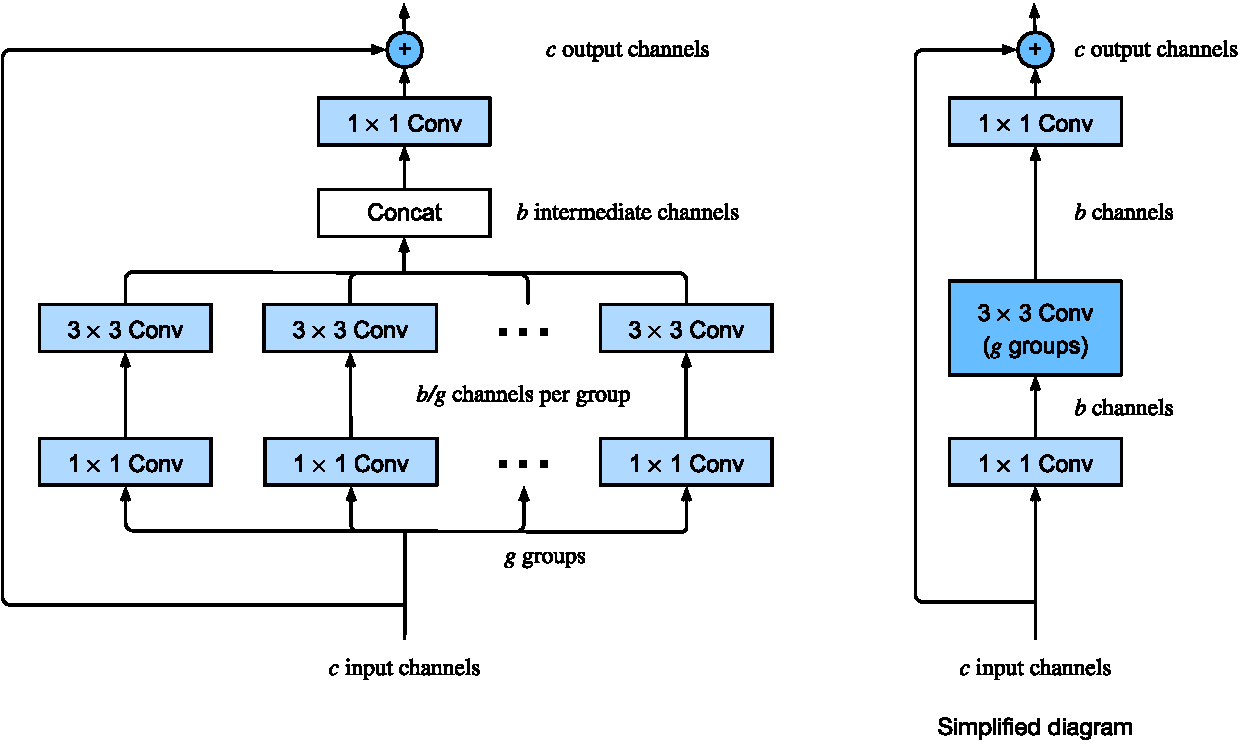
\includegraphics[width = 0.7\linewidth]{resnext-block.pdf}
    \caption{ResNeXt block. Sử dụng tích chập theo nhóm với $g$ nhóm nhanh hơn $g$ lần so với tích chập thông thường. Đây là \textit{bottleneck residual block} khi số lượng kênh trung gian b, nhỏ hơn c. DiveintoDeeplearning}
    \label{fig18}
\end{figure}
\phantom{a}\\\\
ResNeXt là một ví dụ cho cách mà thiết kế các mô hình CNN phát triển theo thời gian: Bằng cách tiết kiệm hơn với tính toán và đánh đổi nó với kích thước của các kích hoạt (số lượng kênh), nó cho phép các mạng nhanh hơn và chính xác hơn với chi phí thấp hơn. Một cách khác để xem các kết cấu được nhóm lại là nghĩ về một ma trận đường chéo khối cho các trọng số tích chập. Lưu ý rằng có khá nhiều 'thủ thuật' như vậy dẫn đến các mạng hiệu quả hơn. Ví dụ, \textit{ShiftNet (Wu et al, 2018)}.\\\\
Chúng ta sẽ thảo luận về một số chiến lược để có được mạng chất lượng cao theo cách tự động hơn sau.
\subsection{Mạng tích chập kết nối dày đặc - DenseNet}
ResNet đã làm thay đổi đáng kể quan điểm về cách tham số hóa của các hàm số trong mạng neuron sâu. Ở một mức độ nào đó, DenseNet có thể được coi là phiên bản mở rộng hợp lý của ResNet. Để đơn giản ta có thể hình dung trực quan rằng DenseNet giống như khai triển Taylor vậy. Nếu ResNet hàm cơ bản chỉ dừng lại ở $f(\textbf{x}) = \textbf{x}$ thì DenseNet hàm cơ bản của nó sẽ ở các hàm cấp cao hơn. Càng đi sâu thì hàm cơ bản càng phức tạp. Các kết nối dày đặc được biểu diễn trong hình \ref{fig19}.
\begin{figure}
    \centering
    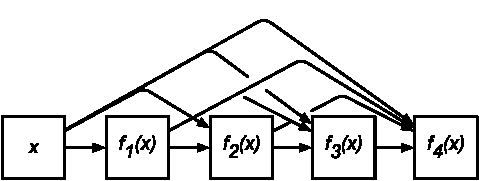
\includegraphics[width = 0.6\linewidth]{densenet.pdf}
    \caption{Các kết nối dày đặc trong DenseNet. DiveintoDeeplearning}
    \label{fig19}
\end{figure}
\phantom{a}\\\\
Giống như ResNet, DenseNet cũng có riêng khối DenseBlock. Khối DenseBlock bao gòn nhiều khối tích chập với cùng số lượng kênh dầu ra. Tuy nhiên ta sẽ nối đầu vào và đầu ra khi tính toàn lan truyền thuận.\\\\
Mỗi khối DenseBlock sẽ làm tăng thêm số lượng kênh. Nhưng việc thêm quá nhiều kênh sẽ tạo nên một mô hình phức tạp quá mức. Do đó, một tầng chuyển tiếp được sử dụng để kiểm soát độ phức tạp của mô hình. Tầng này dùng một tầng tích chập $1\times1$ để giảm số lượng kênh, theo sau là một tầng gộp trung bình với sải bước 2 để giảm một nửa chiều cao và chiều rộng, từ đó giảm độ phức tạp của mô hình hơn nữa.
\subsection{Thiết kế kiến trúc mạng tích chập}
Trong các mục trước chúng ta đã đi một tour về các cấu trúc mạng đã được sử dụng cho Thị giác máy tính. Điểm chung cho tất cả các mạng là nó phụ thuộc rất nhiều vào trực giác của các nhà khoa học.\\\\
Thực tế đã có phương pháp \textit{Neural architecture search} (NAS). Với không gian tìm kiếm cố định, NAS sử dụng chiến lược tìm kiếm để tự động chọn kiến trúc dựa trên ước tính hiệu suất được trả về. Tuy nhiên ta sẽ không bàn luận về nó, bởi nó cần quá nhiều kiến thức và chi phí cũng rất kinh khủng.\\\\
Chúng ta sẽ theo con đường khác, nhẹ nhàng hơn được đề xuất bởi Radosavic (2020), \textit{design network design spaces}. Chiến lược kết hợp sức mạnh của thiết kế thủ công và NAS. Nó thực hiện điều này bằng cách hoạt động trên các bản phân phối mạng và tối ưu hóa các bản phân phối theo cách để có được hiệu suất tốt cho toàn bộ họ mạng.
\subsubsection{Không gian thiết kế AnyNet}
Trước tiên ta cần 1 cái template. Như các mô hình ta đã biết đều có 3 phần: \textit{stem} (gốc), \textit{body} (thân), \textit{head} (ngọn).
\begin{enumerate}
    \item Stem thực hiện xử lý hình ảnh ban đầu, thường thông qua các kết cấu với kích thước cửa sổ lớn hơn
    \item Body bao gồm nhiều khối, thực hiện phần lớn các biến đổi cần thiết để đi từ hình ảnh thô sang biểu diễn đối tượng. Thông qua nhiều stages, và các phép giảm độ phân giải.
    \item chuyển đổi điều này thành các đầu ra mong muốn, chẳng hạn như thông qua hồi quy Softmax để phân loại đa lớp
\end{enumerate}
Trong AnyNet ta sẽ sử dụng khối ResNeXt đã đề cập ở trên (hình \ref{fig20}).
\begin{figure}
    \centering
    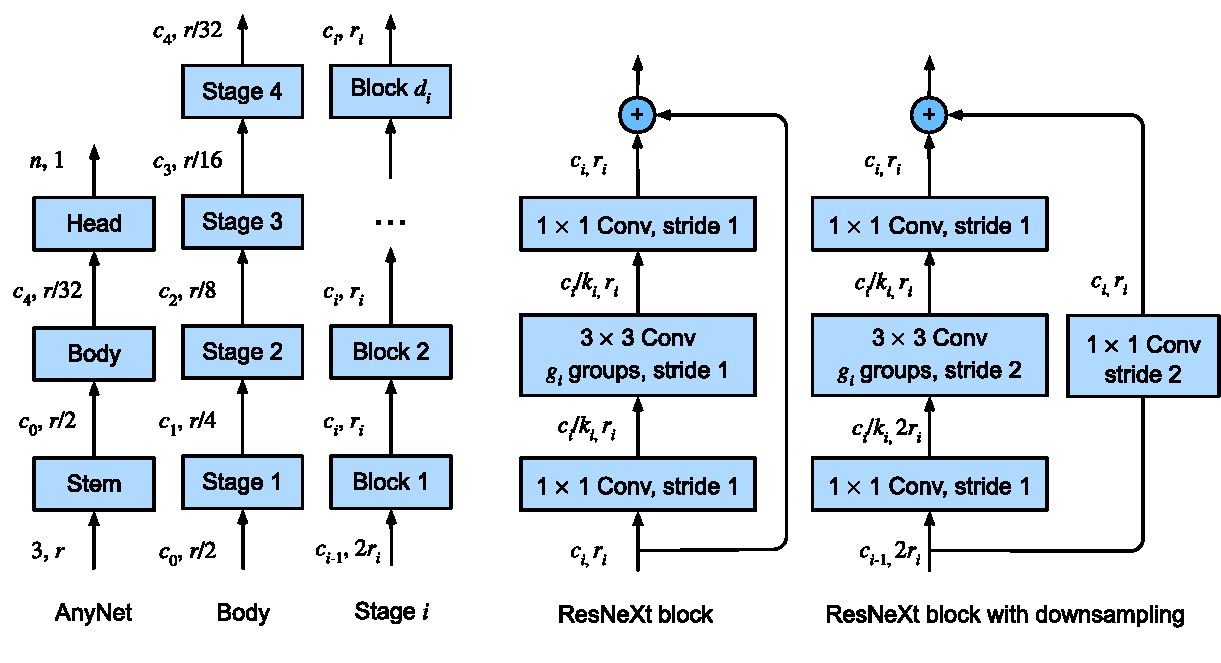
\includegraphics[width = 0.7\linewidth]{anynet.pdf}
    \caption{Không gian thiết kế AnyNet. $(c,r)$ dọc theo các mũi tên là số lượng kênh và độ phân giải tại đó. từ trái qua phải: cấu trúc mạng tổng quát bao gồm stem, body, và head. Hai cấu trúc khối thay thế cho nhau, một giảm một nửa ở đầu ra và còn lại không. Thiết kế bao gồm chiều sâu $d_i$, số kênh đầu ra $c_i$, số lượng nhóm $g_i$ và tỉ lệ bottleneck $k_i$ cho từng stage. DiveintoDeeplearning}
    \label{fig20}
\end{figure}
\subsubsection{Phân phối và tham số của không gian thiết kế}
Phần này khá phức tạp, chung quy lại qua các thử nghiệm (hình \ref{fig21}) ta thu được kết luận như sau:
\begin{enumerate}
    \item tỉ lệ bottleneck không ảnh hưởng đến hiệu quả. Chọn $k_i = k$ cho tất cả các stage.
    \item số lượng nhóm cũng không ảnh hưởng đến hiệu quả. Chọn $g_i = g$ cho tất cả các stage.
    \item Tăng $c_i$ qua mỗi stage.
    \item Tăng $d_i$ qua mỗi stage.
\end{enumerate}
\begin{figure}
    \centering
    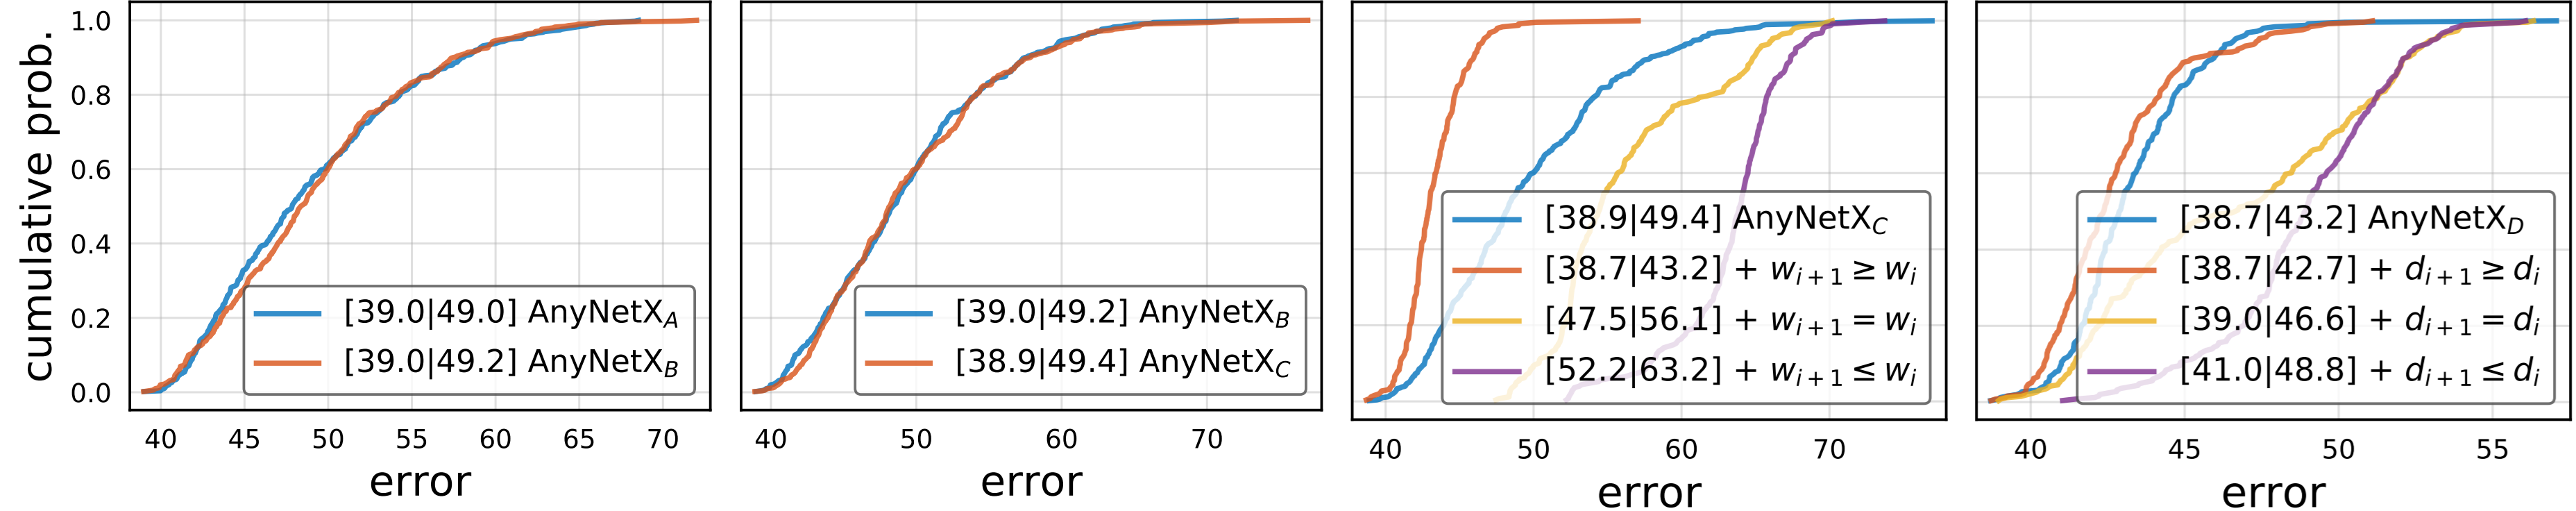
\includegraphics[width = 0.8\linewidth]{regnet-fig.png}
    \caption{So sánh các hàm phân phối lỗi thực nghiệm của các không gian thiết kế. AnyNetA là thiết kế ban đầu, AnyNetB gắn với tỉ lệ bottleneck, AnyNetC gắn với số nhóm, AnyNetD tăng chiều sâu qua từng stage. Từ trái qua phải: (i) tỉ lệ bottleneck không ảnh hưởng đến kết quả, (ii) số lượng nhóm cũng không ảnh hưởng, (iii) tăng số kênh, cải thiện kết quả, (iv) tăng chiều sâu từng chặng cũng cải thiện kết quả. DiveintoDeeplearning}
    \label{fig21}
\end{figure}
\section{Hạn chế của CNN}
CNN thật sự là một cuộc cách mạng, đã và đang đạt được nhiều thành tựu ấn tượng. Tuy nhiên chúng cũng có nhiều hạn chế, đó là một trong những lí do, không phải ai, công ty hay doanh nghiệp nào cũng muốn sử dụng CNN. Có thể kể ra vài hạn chế ở đây:\begin{enumerate}
    \item Đầu tiên là "hộp đen", chúng ta thật sự không hiểu được hoàn toàn về CNN, cũng không thể giải thích chính xác tại sao nó lại tốt đến vậy.
    \item Nó cần quá nhiều Data để đạt được hiệu quả, và phụ thuộc vào GPUs.
    \item Tỏ ra yếu kém với các dữ liệu chất lượng thấp
    \item CNN chỉ có thể phân cụm các pixels tạo thành các đặc trưng lớn (hình \ref{fig22}). Nhưng không thật sự hiểu về sự hiện diện của các vật thể (\ref{fig23})
\end{enumerate}
\begin{figure}
    \centering
    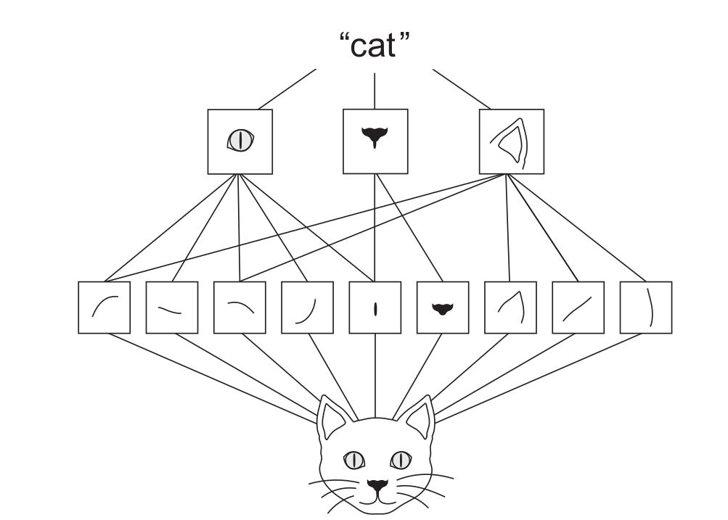
\includegraphics[width = 0.8\linewidth]{download (1).jpg}
    \caption{Đơn giản CNN}
    \label{fig22}
\end{figure}
\begin{figure}
    \centering
    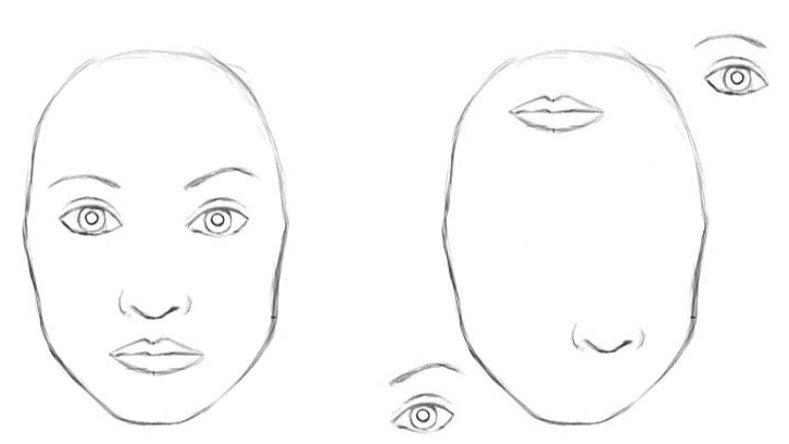
\includegraphics[width = 0.6\linewidth]{download (2).jpg}
    \caption{CNN không hiểu được sự hiện diện của vật thể trong một bức ảnh. Hai bức ảnh này đều cho cùng 1 kết quả nếu sd CNN, mặc dù rõ ràng hình phải không phải mặt người.}
    \label{fig23}
\end{figure}
\phantom{a}\\\\
Có thể lấy lí do là ở tầng gộp (Pooling). Tầng gộp không giữ thông tin về vị trí tương đối giữa các vật thể với nhau, cứ giả sử như ở MaxPooling, MaxPooling chỉ lấy các neuron active nhất (hay có giá trị lớn nhất) và đưa cho các layer tiếp theo. Việc này tuy giảm kích thước của feature maps nhưng lại làm mất đi thông tin quý giá về không gian giữa các feature khi dữ liệu đi qua các layers.\\\\
Để khắc phục việc này, Geoffrey Hinton và các cộng sự đã đề xuất \textit{Capsule Network}. Một nhóm các neuron mà các vector của nó được dùng để biểu diễn các tham số của một entity (thực thể) nhất định như một object hay một phần của object đó.\\\\
CapsNet lấy ý tưởng từ một quá trình trong \textit{Computer Graphics} gọi là \textit{Rendering}: Từ các thông tin về vật thể như vị trí, khích thước, cấu tạo, chiếu sáng, bóng đổ, \ldots để hiện thị ra hình ảnh của đối tượng lên màn hình. Hnton suy đoán rằng, cách thức não bộ của con người nhận diện ra một vật thể có thể là quá trình ngược lại với \textit{Rendering}. Ông gọi đó là \textit{Inverse Graphics}, được hiểu là khi mắt nhìn một vật thể, chúng phân tách vật thể thành các features, và cố gắng match chúng với các features và mối quan hệ giữa chúng đã được học từ trước được lưu ở trong não.
\begin{figure}
    \centering
    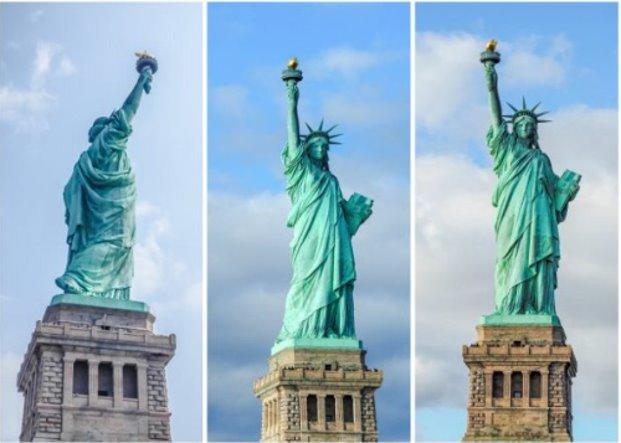
\includegraphics[width = 0.6\linewidth]{download (3).jpg}
    \caption{Inverse Graphics. nếu chúng ta trước đó chỉ nhìn thấy một trong ba bức ảnh trên, sau đó nếu ta nhìn thấy hai bức ảnh còn lại thì ta vẫn có thể đoán nhận ra chúng là ảnh chụp của cùng một bức tượng, dù cho chúng có được chụp ở các góc độ khác nhau.}
    \label{fig24}
\end{figure}
\section{Tinh chỉnh (Fine-tuning)}
Trong thực tế không phải dữ liệu nào cũng mạnh như ImageNet, do đó tất yếu mô hình sẽ không đạt được kết quả cao nhất trên các tập dữ liệu nhỏ. Giải pháp đơn giản là thu thập thật nhiều dữ liệu, song điều này lại rất mất thời gian và chi phí (ImageNet đã sử dụng hàng triệu đô la từ nguồn tài trợ nghiên cứu). Một giải pháp khác là học truyền tải (\textit{transfer learning}), mang kiến thức đã học từ dữ liệu gốc sang tập dữ liệu mục tiêu. Có thể các đặc trưng của tập dữ liệu mới đã có thể được trích xuất trong quá trình huấn luyện ImageNet\\\\
Fine-tuning, một kĩ thuật đơn giản trong học truyền tải. Việc tinh chỉnh được tiến hành theo các bước sau:
\begin{enumerate}
    \item Tiền huấn luyện một mô hình mạng nơ-ron, tức là là mô hình gốc, trên tập dữ liệu gốc (chẳng hạn tập dữ liệu ImageNet).
    \item Tạo mô hình mạng nơ-ron mới gọi là mô hình mục tiêu. Mô hình này sao chép tất cả các thiết kế cũng như các tham số của mô hình gốc, ngoại trừ tầng đầu ra. Ta giả định rằng các tham số mô hình chứa tri thức đã học từ tập dữ liệu gốc và tri thức này sẽ áp dụng tương tự đối với tập dữ liệu mục tiêu. Ta cũng giả định là tầng đầu ra của mô hình gốc có liên hệ mật thiết với các nhãn của tập dữ liệu gốc và do đó không được sử dụng trong mô hình mục tiêu.
    \item Thêm vào một tầng đầu ra cho mô hình mục tiêu mà kích thước của nó là số lớp của dữ liệu mục tiêu, và khởi tạo ngẫu nhiên các tham số mô hình của tầng này.
    \item Huấn luyện mô hình mục tiêu trên tập dữ liệu mục tiêu, chẳng hạn như tập dữ liệu ghế. Chúng ta sẽ huấn luyện tầng đầu ra từ đầu, trong khi các tham số của tất cả các tầng còn lại được tinh chỉnh từ các tham số của mô hình gốc.
\end{enumerate}
\begin{figure}
    \centering
    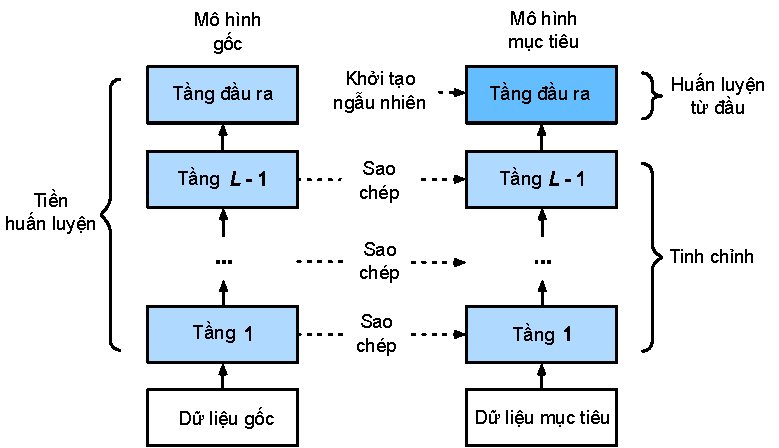
\includegraphics[width = 0.7\linewidth]{finetune.pdf}
    \caption{Thực hiện tinh chỉnh}
    \label{fig25}
\end{figure}

\section{Mã nguồn}
Mã nguồn của phần này có thể tìm thấy ở đây: \\\url{https://github.com/thuantn210823/Computer-Vision-IPSAL-LAB-}

\section{Tài liệu tham khảo}
    \begin{thebibliography}{9}
        \bibitem{slide}
        Truong. PV, Thao. TT Bài giảng , Đại học Bách Khoa Hà Nội.
        \bibitem{book}
        Aston Zhang, Zachary C.Lipton, Mu Li, and Alexander J. Smola \emph{Dive into Deep Learning}.
        \bibitem{website}
        \url{d2l.aivivn.com}
        \bibitem{website}
        \url{https://blog.vietnamlab.vn/capsule-networks/}
        \bibitem{website}
        \url{https://iq.opengenus.org/disadvantages-of-cnn/}
        \bibitem{website}
        \url{https://arxiv.org/pdf/1710.09829v2.pdf}
        \bibitem{website}
        \url{https://www.engati.com/glossary/convolutional-neural-network#:~:text=Some%20of%20the%20disadvantages%20of,classifying%20images%20with%20different%20positions.}

    \end{thebibliography}
\end{document}
